\clearpage

\section {Results of the $\bar{\nu}_{e}$-appearance analysis with the Run 5+6 dataset}
\label{sec:results}

%--------------------------------------------------------------------------------------
% p-value
%--------------------------------------------------------------------------------------

\subsection {Significance to $\bar{\nu}_e$ appearance}
\label{sec:results_bestfit}

The rate-only and rate+shape p-values for $\bar{\nu}_e$-appearance are performed
on the combined \TotalPot{} POT Run 5+6 dataset 
following the same procedure as in section~\ref{sec:sensitivity}. 
1-sided p-values are computed on the right tail of the test statistic expected distribution.
All the \NSyst{} systematic parameters are marginalized.
Only the oscillation parameters $\sin^2 \theta_{12}$ and $\Delta m^2_{21}$ are fixed to their nominal values.
In figure~\ref{fig:ereco_expVsdata} the expected reconstructed energy distribution is compared with data.
A summary of the observed number of events in SuperK, $\Delta \chi^{2}$ and p-values is given
in table~\ref{tab:results}.

%...........................................................
%
% Ereco expected with data overlapped
%

\begin{figure}
\center
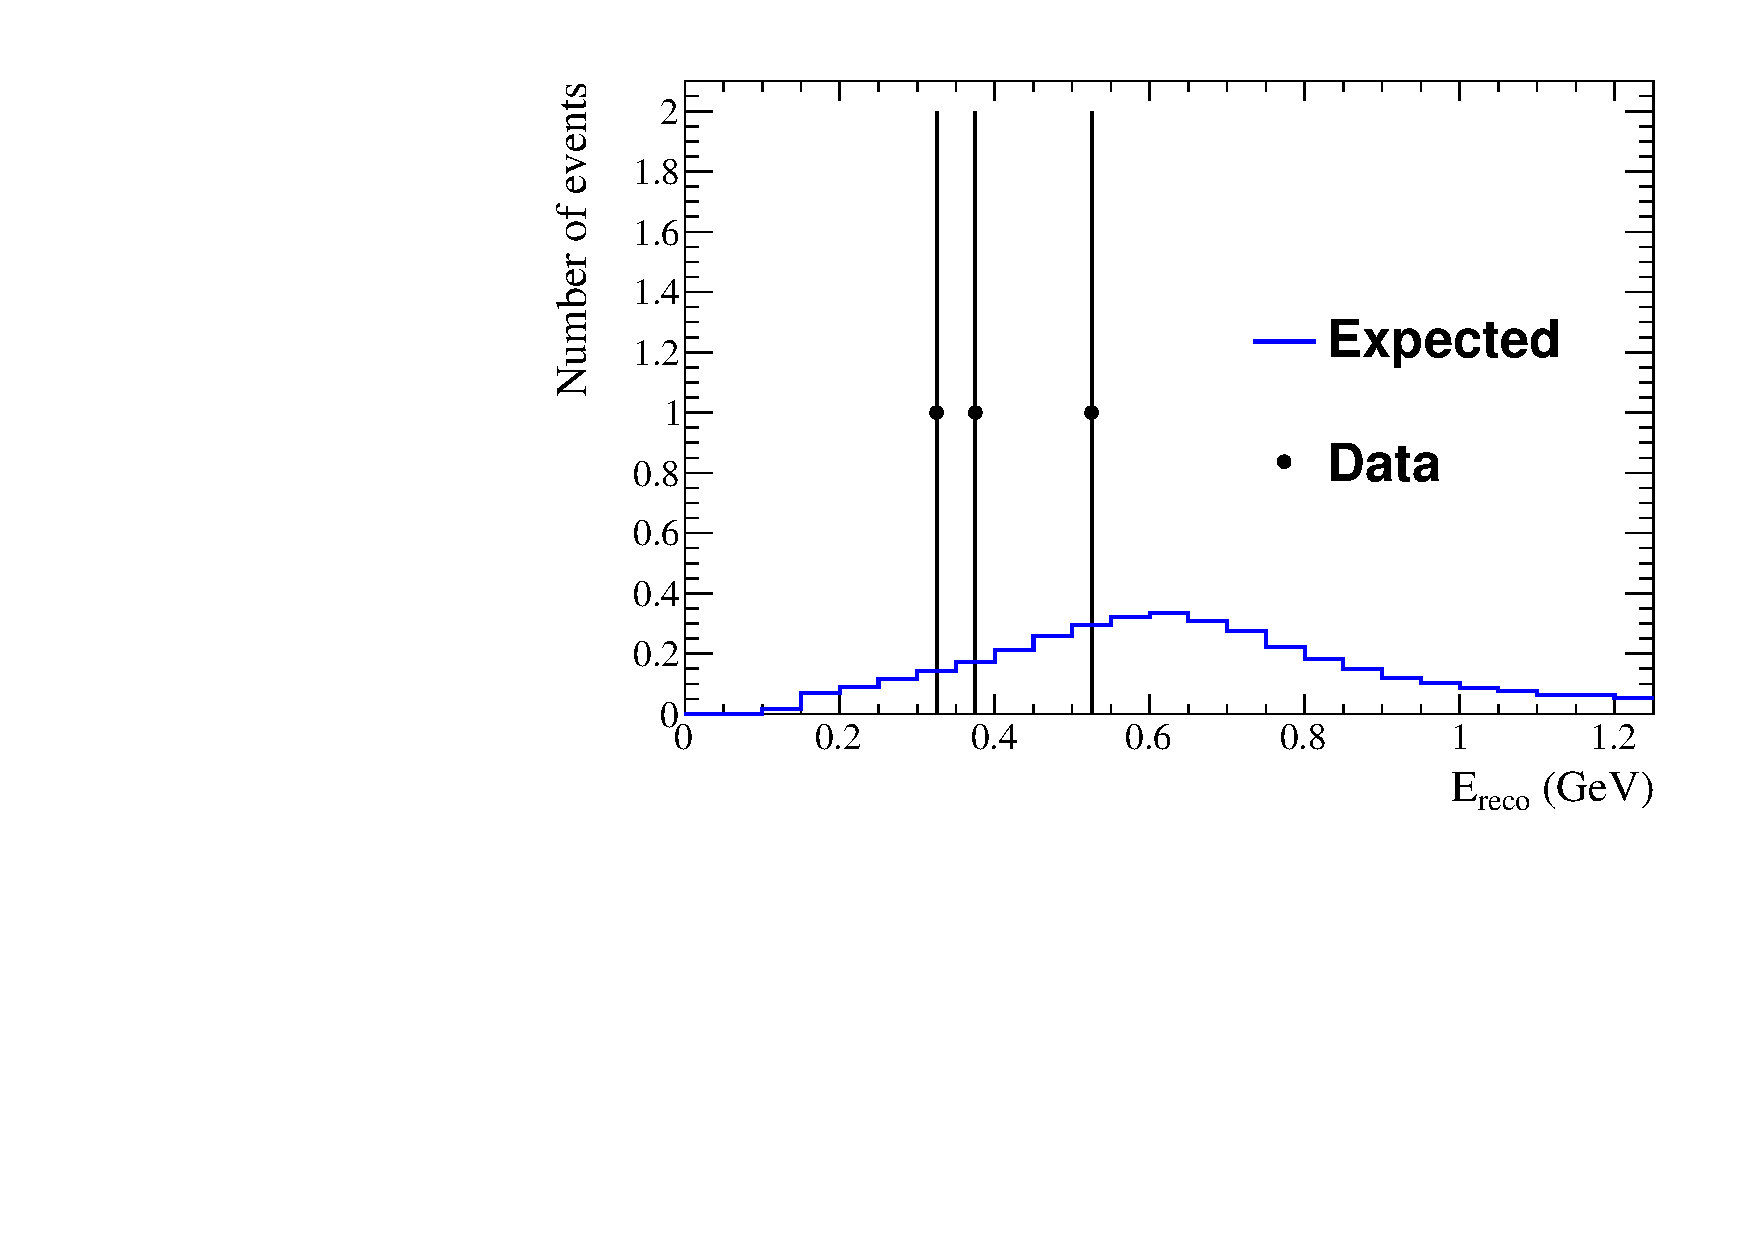
\includegraphics[width=0.48\linewidth]{./nuebar_plots/results/ereco_dataVsexp.pdf}
\caption {
The expected reconstructed energy distribution (blue) is compared to the Run 5+6 dataset (black dots),
which corresponds to \TotalPot POT.
The expected distribution corresponds to the oscillation parameters shown in table~\ref{tab:osc_params_fixed_values_reactor}.
}
\label{fig:ereco_expVsdata}
\end{figure}



%...........................................................
%
% Delta Chisq and # of events distributions with data overlapped
%

\begin{figure}
\center
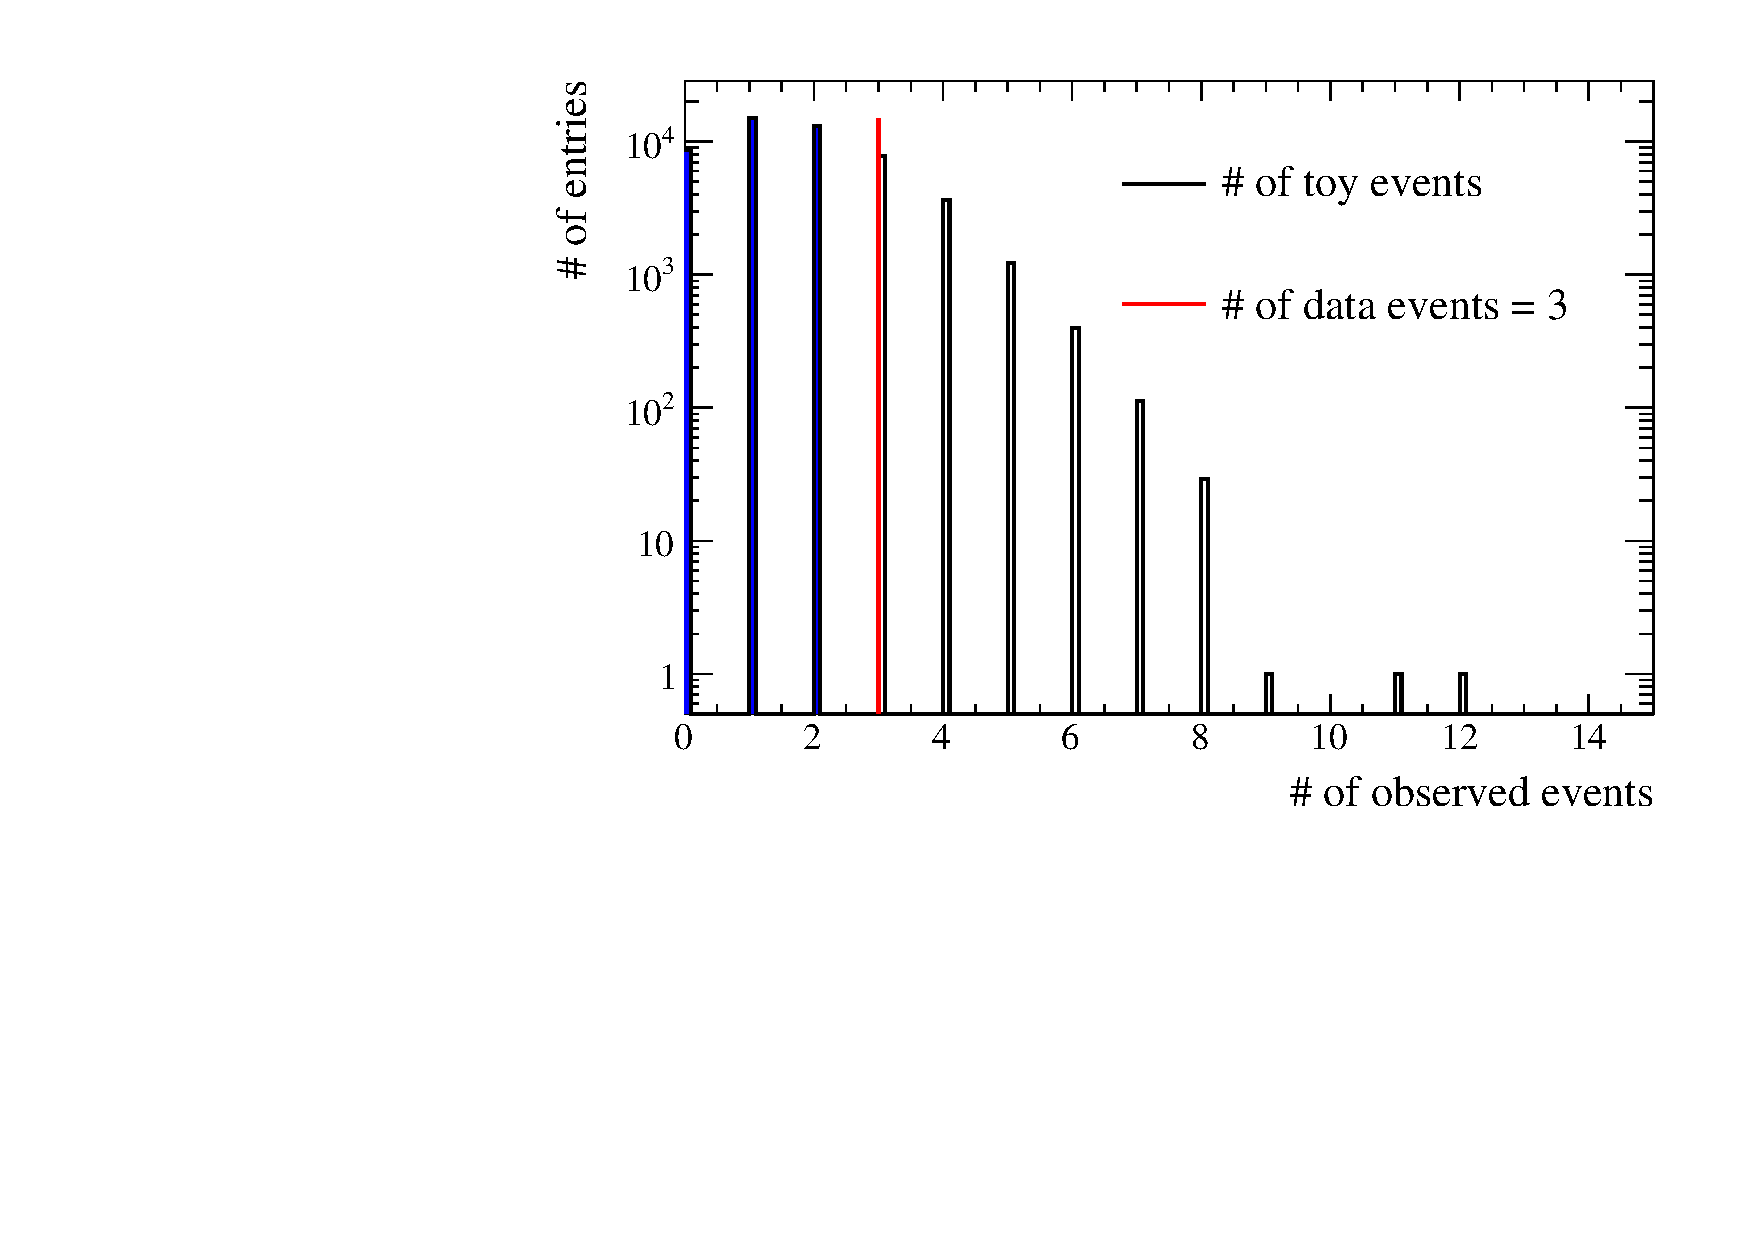
\includegraphics[width=0.48\linewidth]{./nuebar_plots/results/pvalue_rateonly_50ktoys}
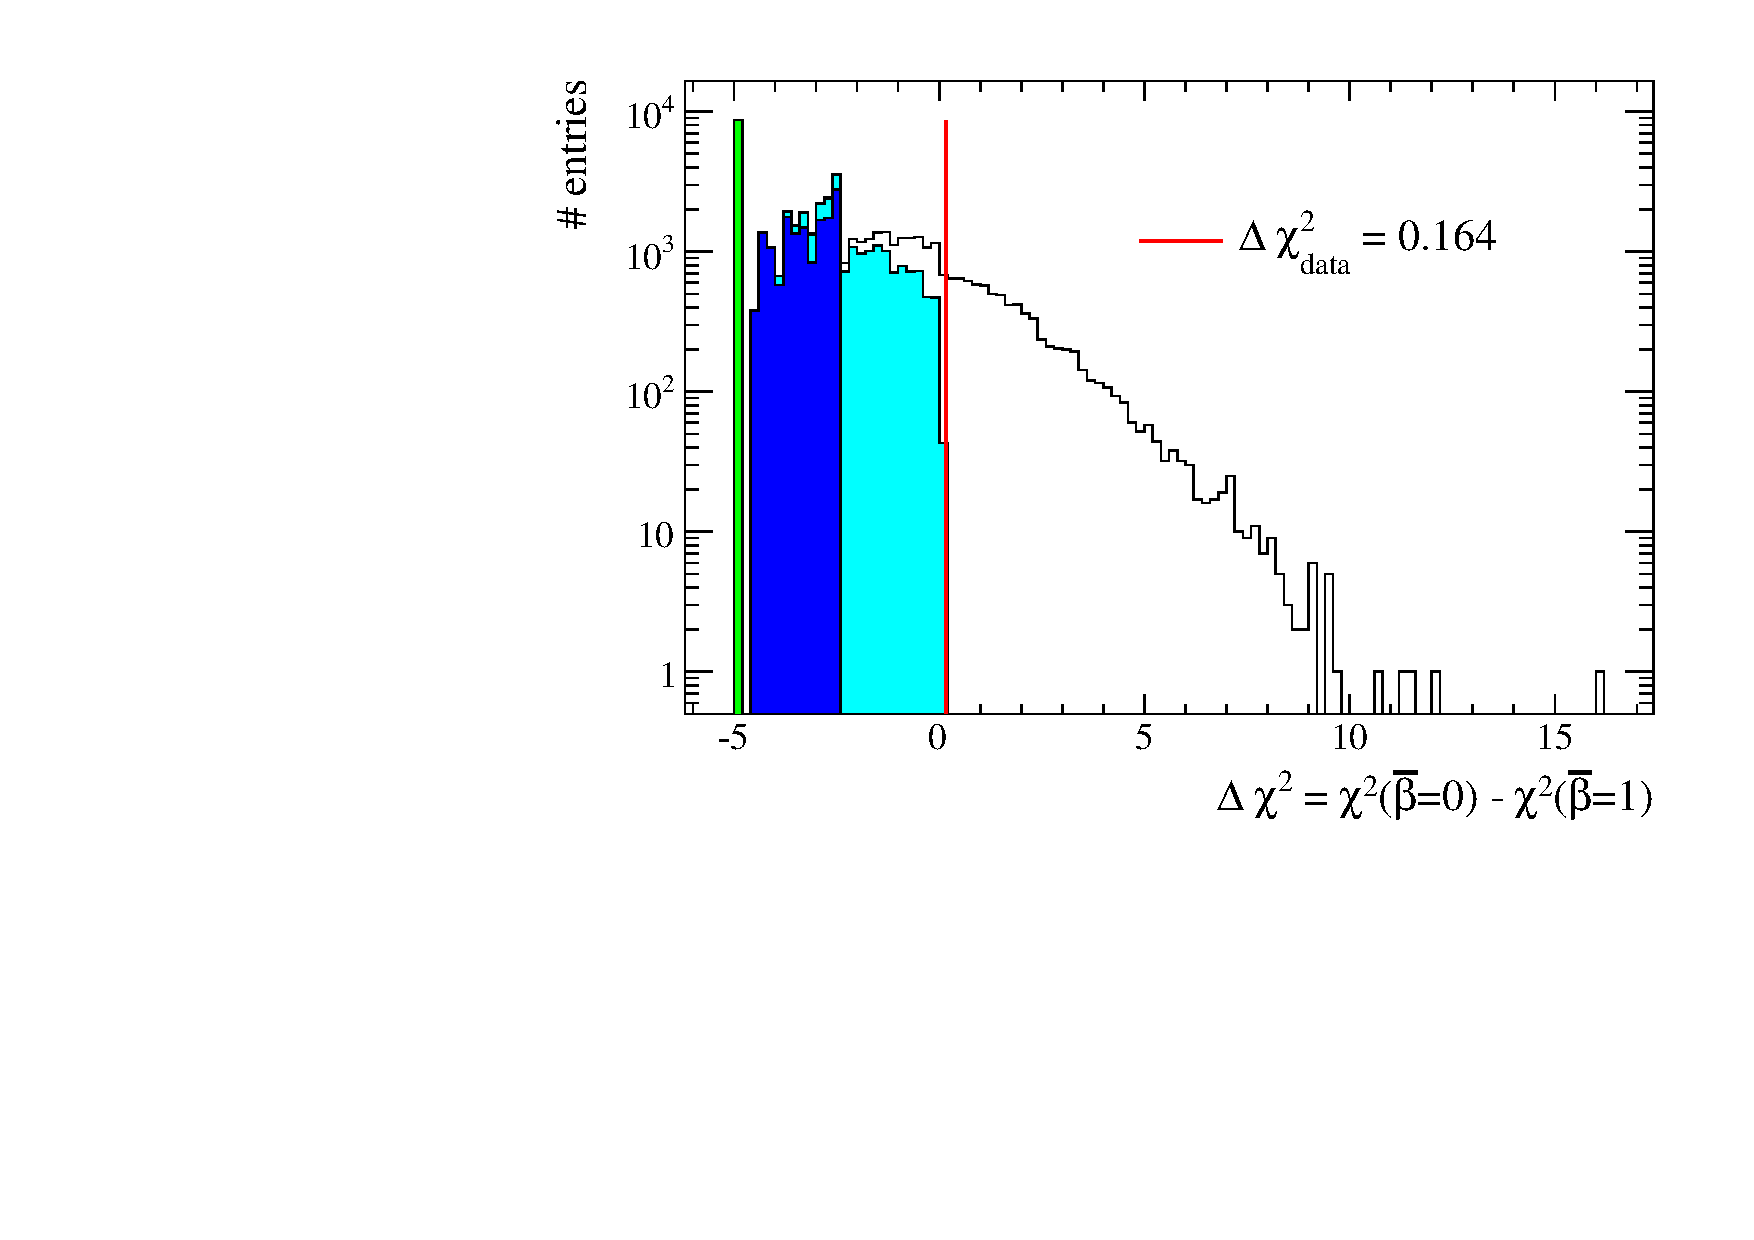
\includegraphics[width=0.48\linewidth]{./nuebar_plots/results/pvalue_rateshape_50ktoys}
\caption {
The distribution of the total number of events from each of the \NumToysLarge toy experiments. 
The red line corresponds to the total number of events (left) and $\Delta \chi^2$ (right) given by the Run 5+6 dataset. 
Data correspond to \TotalPot POT.
The distribution of the test statistics are obtained by performing 50k toys. 
%\FakePotLow POT (left) and \FakePotHigh (right).
}
\label{fig:pvalue_rateonly_data}
\end{figure}


%...........................................................
%
% Table summarizing p-value for different test statistics
%
\begin{table}[htb]
\centering
\begin{tabular}{| c | c | c | c | c | c |}
\hline
Observed num. of events 		& p-value (rate-only)	 	& $\chi^2 (\beta=0)$ 		& $\chi^2 (\beta=1)$	 	& $\Delta \chi^2$ 	& p-value (rate+shape)  	\\
\hline
3				 		& 0.2637 		 		& 11.6405				& 11.4763				& 0.164213		 	& 0.1589			  	\\
\hline
\end{tabular}
\caption{
Summary of observed number of events, $\chi^2$ for $\beta=0$ and $\beta=1$, $\Delta \chi^2$, rate-only and rate+shape p-values from the combined Run 5+6 dataset.
The quoted $\chi^2$ values were computed from Eq.~\ref{eq:loglikemarg},
while $\Delta \chi^2$ from eq.~\ref{eq:deltachisq_rateshape} in Sec.~\ref{sec:oscfit_method}.
using the reconstructed energy binning scheme given in Sec.~\ref{sec:mc_templates:template_binning}.
The p-values are obtained performing 50k toys with $\beta=0$ in order to get the distribution of the test statistic.
}
\label{tab:results}
\end{table}


%...........................................................
%
% Discussion about the p-value
%

The distribution of the expected test statistics, compared with the one obtained from the Run5-6 dataset, is shown in figure~\ref{fig:pvalue_rateonly_data}.
In figure~\ref{fig:ereco_expVsdata_components} the signal and background components are shown 
separately and compared to the data. On the left plot both shape and normalization informations are shown,
while on the right plot only shape informations are given.
The observed event at about 0.53 GeV is in the region where the $\bar{\nu}_{\mu} \to \bar{\nu}_e$ signal is larger than the background.
Indeed in that region the $\bar{\nu}_{\mu} \to \bar{\nu}_e$ signal is about the 60\% and shows its maximum.
The other 2 observed events, with a reconstructed energy of about 0.35 GeV and 0.36 GeV are in a region where
the background starts to become dominant.

\begin{figure}
\center
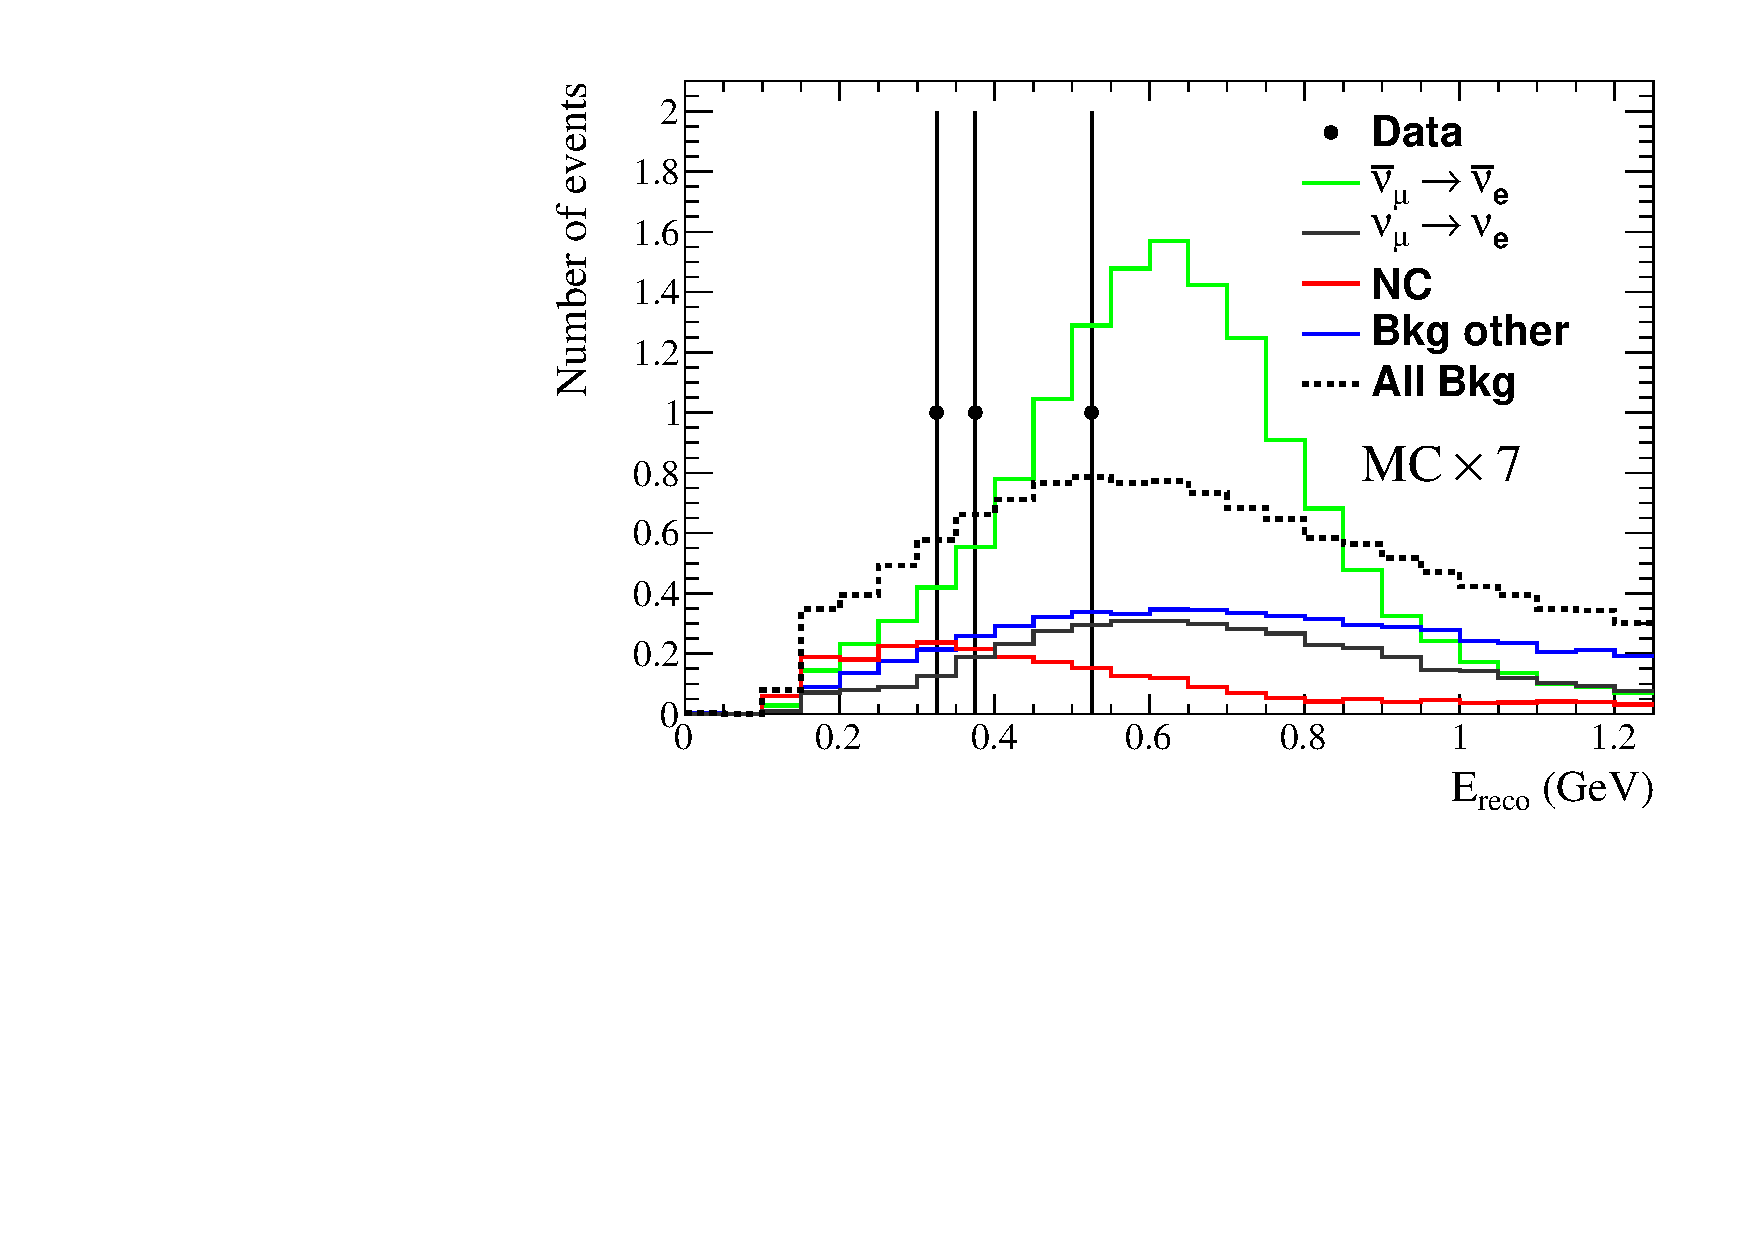
\includegraphics[width=0.48\linewidth]{./nuebar_plots/results/ereco_dataVsexp_splitted_MCx7.pdf}
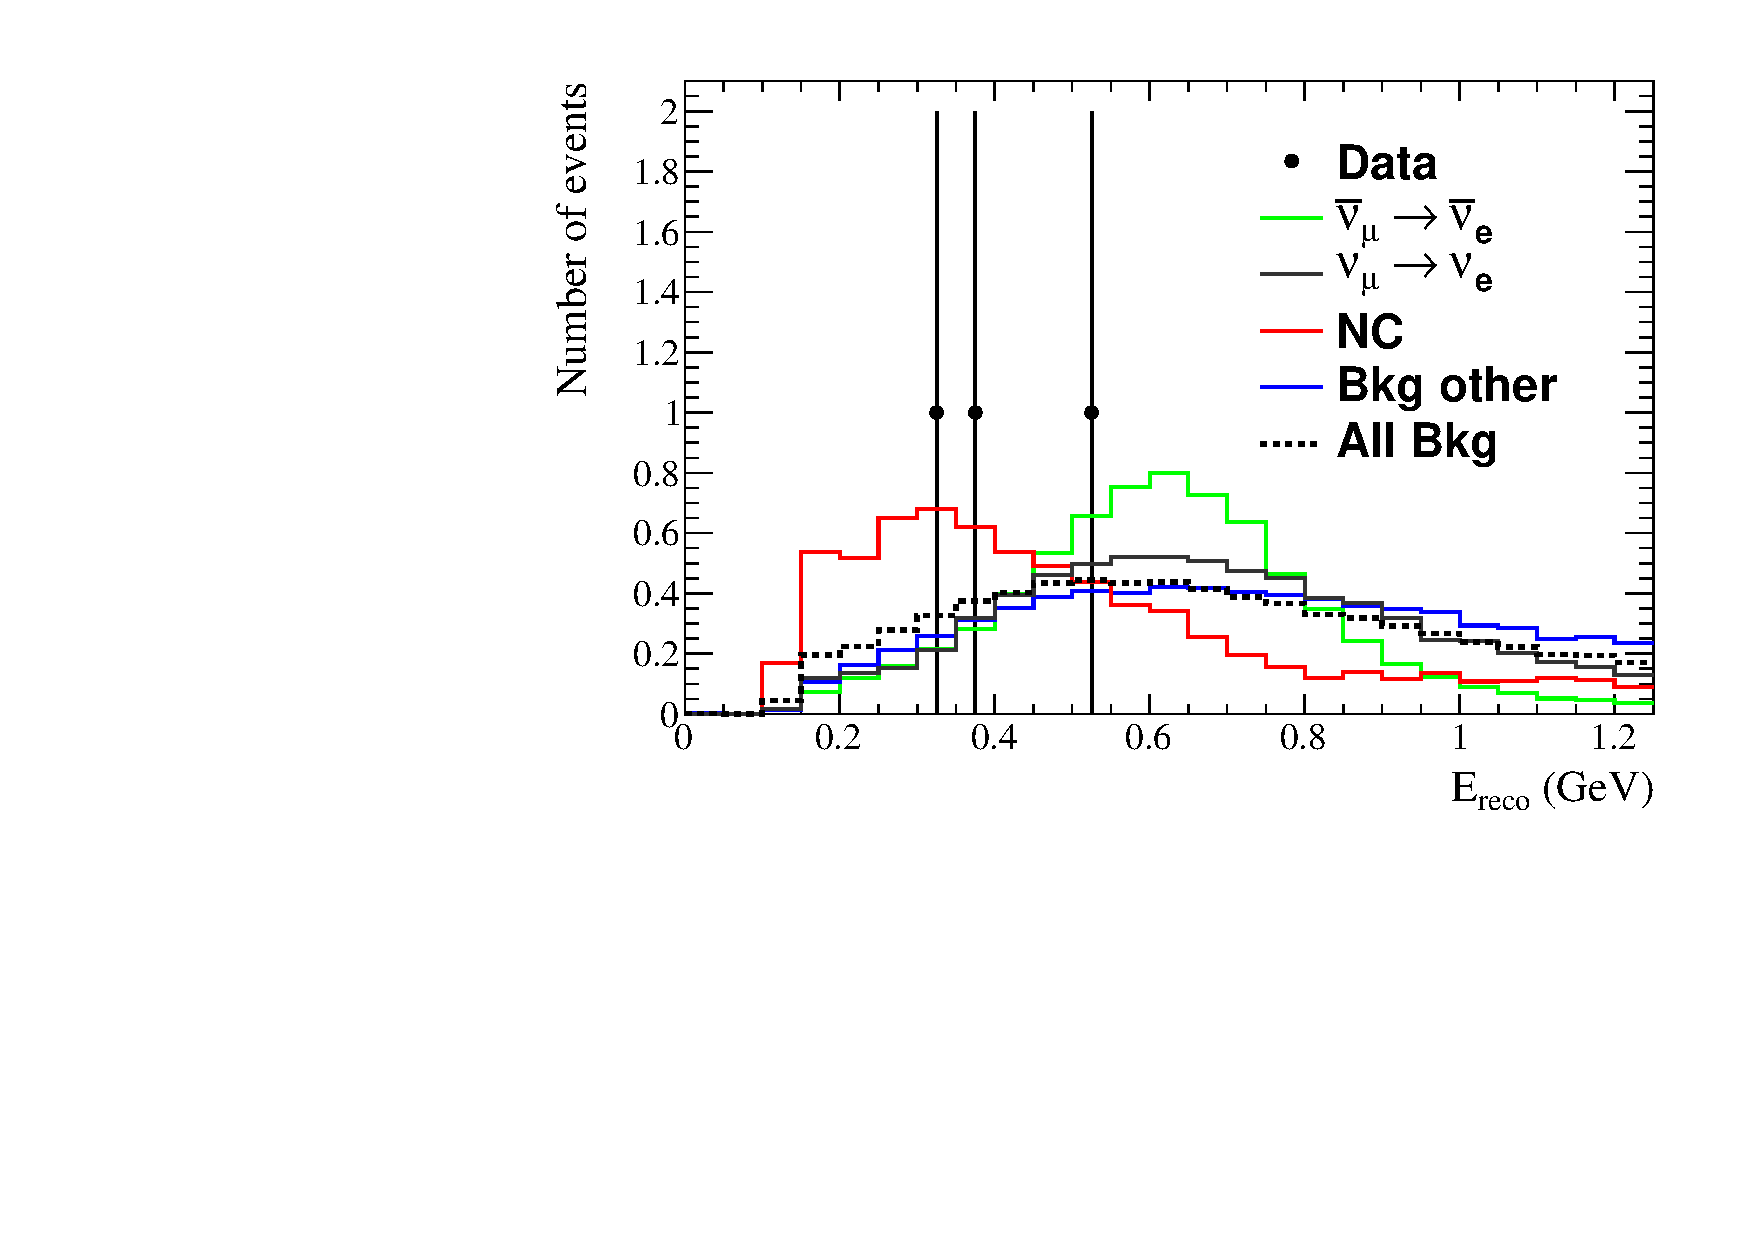
\includegraphics[width=0.48\linewidth]{./nuebar_plots/results/ereco_dataVsexp_splitted_MCx7_normarea.pdf}
\caption {
Predicted reconstructed-energy spectrum components of 1 $e$-like ring events
from various true neutrino reaction modes,
in antineutrino beam mode with oscillations.
The following components are shown separately:
$\bar{\nu}_{\mu} \to \bar{\nu}_e$ signal (green), 
$\nu_{\mu} \to \nu_e$ background (grey), 
NC (red) background, 
background other (blue) and all background components.
The spectrum was generated using the BANFF postfit MC templates.
Each component is separately shown.
The spectrum shown was generated assuming the normal hierarchy and the oscillation parameters in table~\ref{tab:osc_params_fixed_values_reactor}.
The black dots correspond to Run 5+6 dataset (\TotalPot POT).
On the left plot each component is first normalized to \TotalPot POT and then rescaled of a factor 7 in order to better compare with data.
On the right plot each component is first normalized to its area and then rescaled by a factor 7. 
}
\label{fig:ereco_expVsdata_components}
\end{figure}



%...........................................................
%
% Delta Chisq and # of events distributions with data overlapped signal and bkg
%

In figure~\ref{fig:pvalue_rateonly_sigbkg} and figure~\ref{fig:pvalue_rateshape_sigbkg}
the distributions of the test statistic, for rate-only and rate+shape analyses, are shown and compared with the data.
It is already clear that the current dataset is compatible with both $\beta=0$ and $\beta=1$, since the 
significance for both cases is not large enough.

\begin{figure}
\center
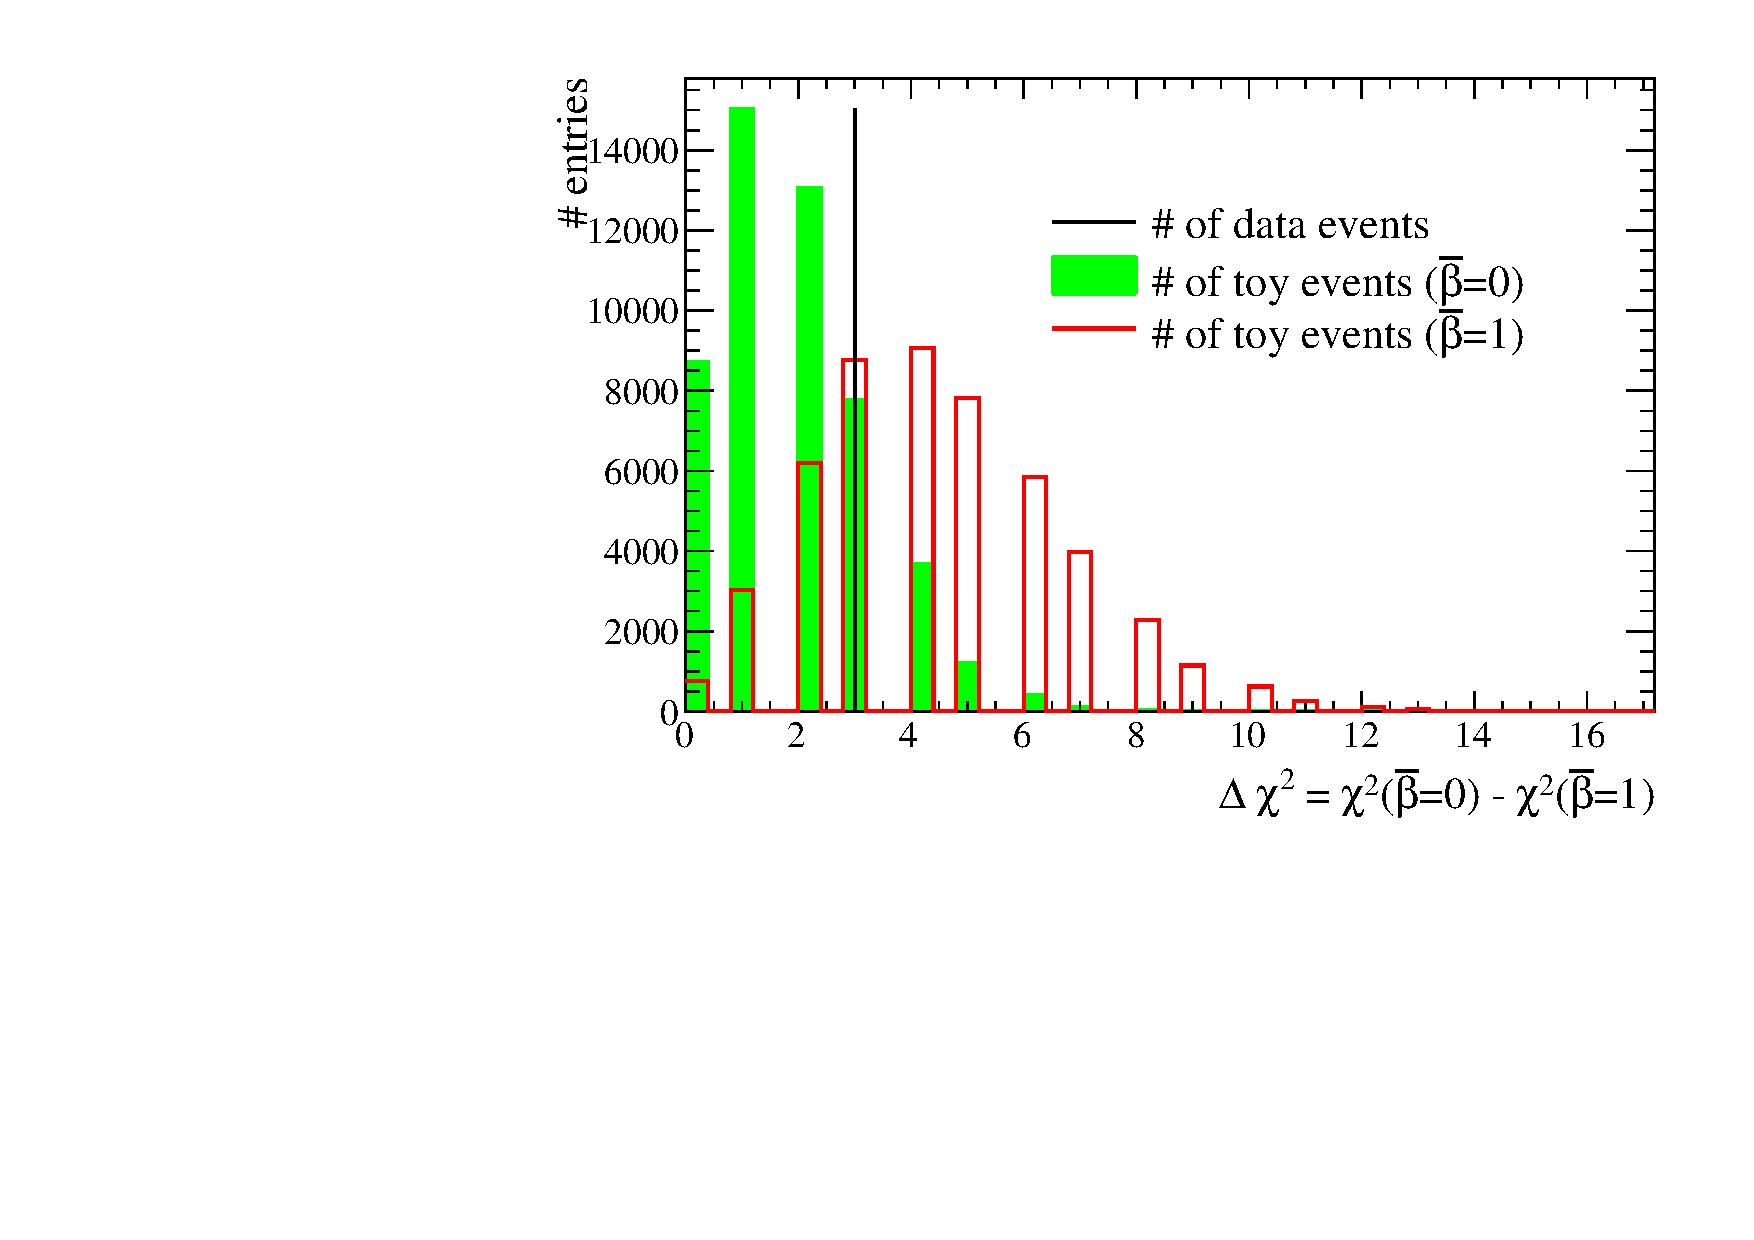
\includegraphics[width=0.48\linewidth]{./nuebar_plots/results/pvalue_rateonly_sigbkg_50ktoys.pdf}
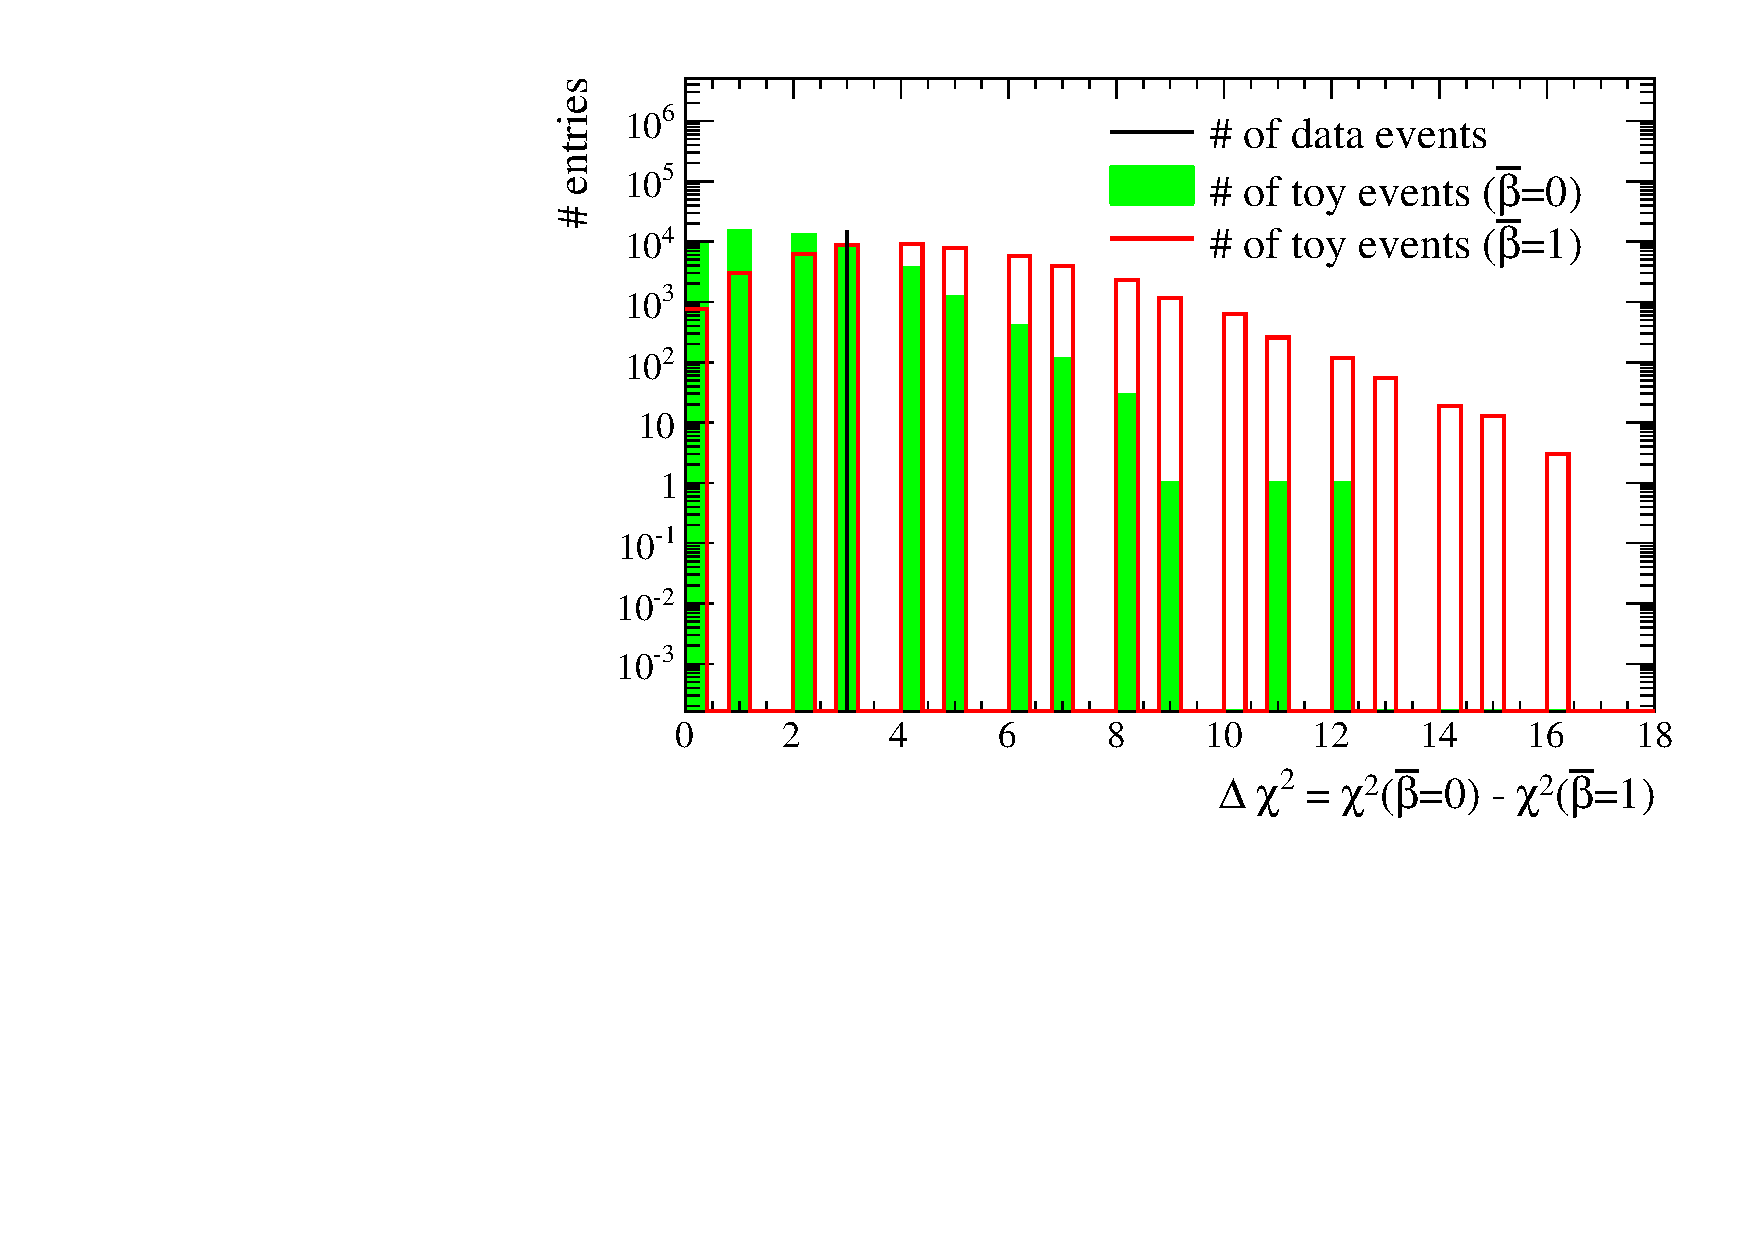
\includegraphics[width=0.48\linewidth]{./nuebar_plots/results/pvalue_rateonly_sigbkg_50ktoys_log_zoom.pdf}
\caption {
The distribution of the total number of events from each of the \NumToysLarge toy experiments is
shown for both $\beta=0$ (green) and $\beta=1$ (red).
The black line corresponds to the total number of events observed in the Run 5+6 dataset. 
Data correspond to \TotalPot POT.
Both linear (left) and logarithmic (right) scales are shown.
}
\label{fig:pvalue_rateonly_sigbkg}
\end{figure}

\begin{figure}
\center
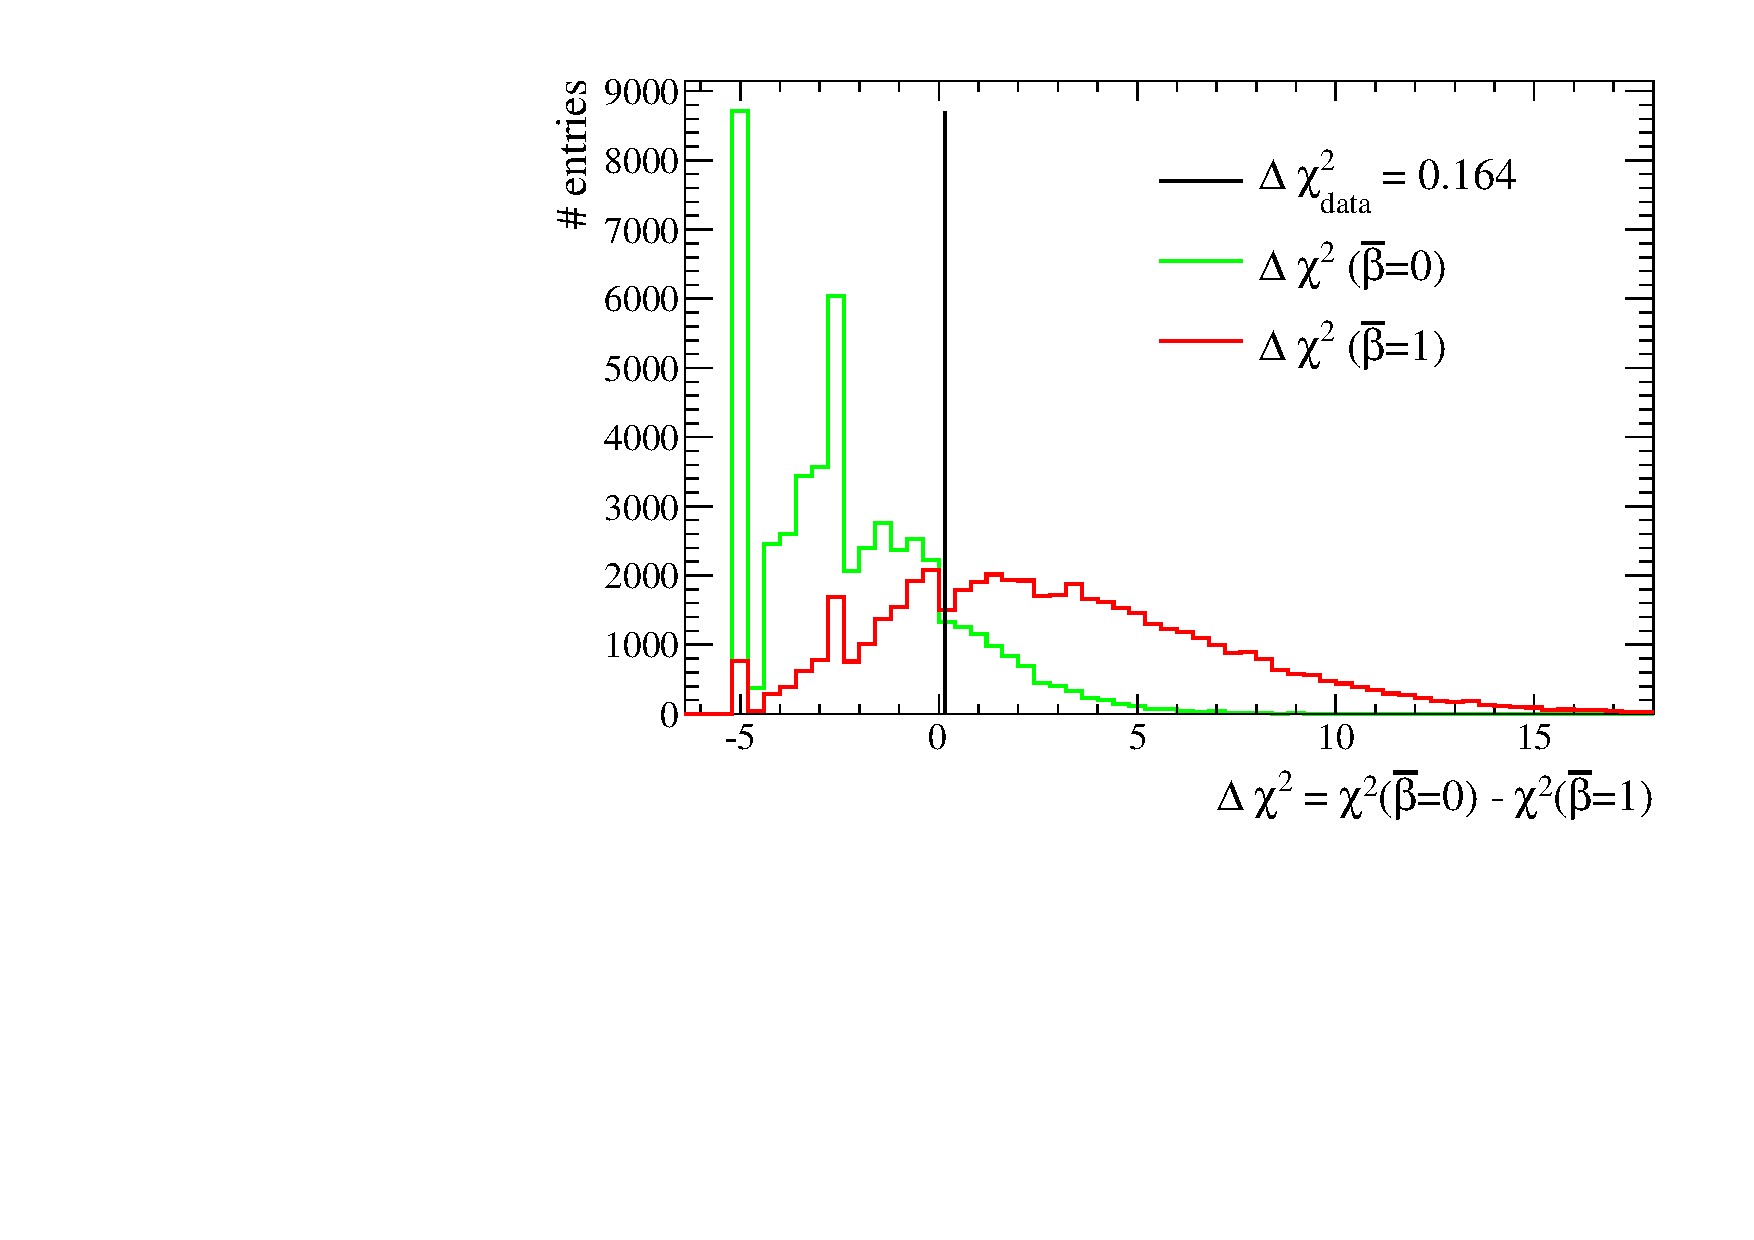
\includegraphics[width=0.48\linewidth]{./nuebar_plots/results/pvalue_rateshape_sigbkg_50ktoys.pdf}
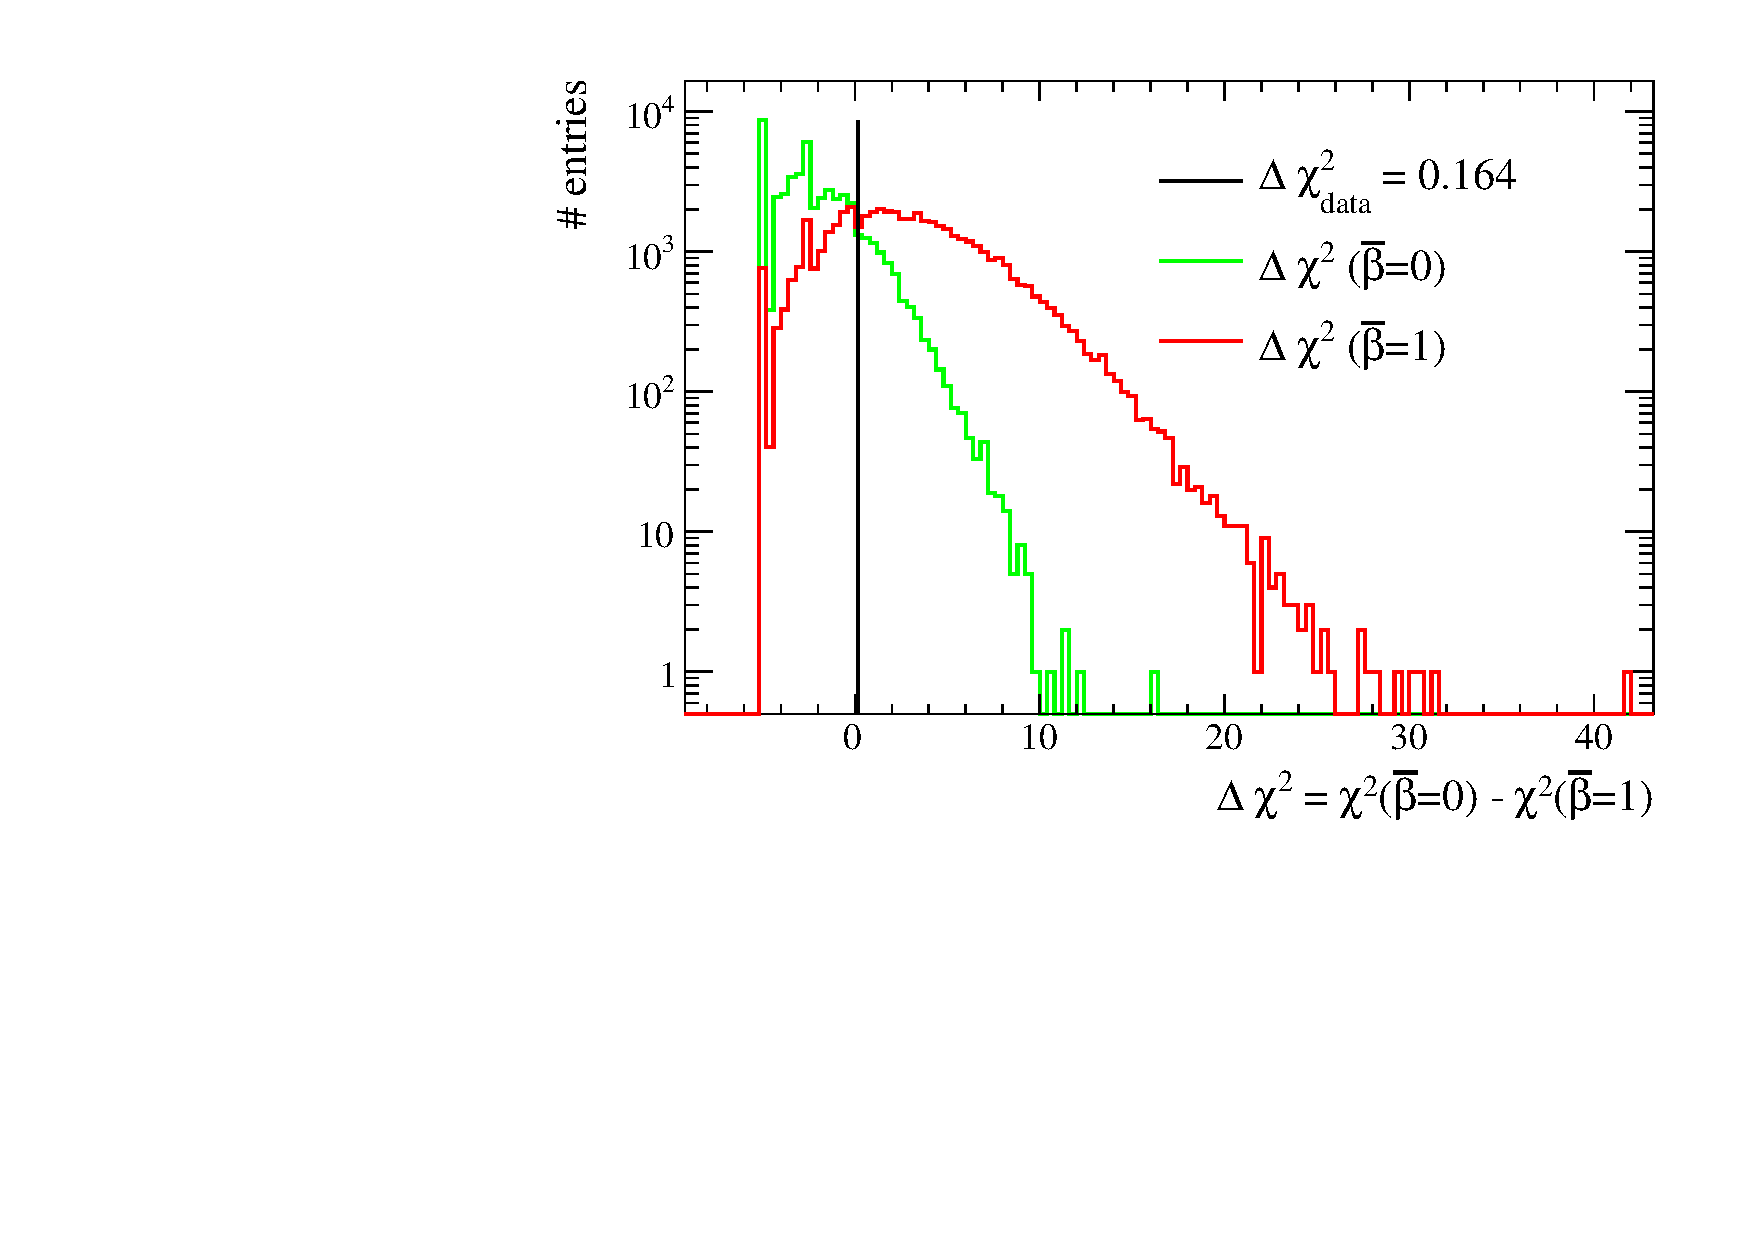
\includegraphics[width=0.48\linewidth]{./nuebar_plots/results/pvalue_rateshape_sigbkg_50ktoys_log.pdf}
\caption {
The distribution of the test statistic $\Delta \chi^2$ for each of the \NumToysLarge toy experiments is shown for
both $\beta=0$ (green) and $\beta=1$ (red). 
The black line corresponds to the $\Delta \chi^2$ obtained from the Run 5+6 dataset. 
Data correspond to \TotalPot POT.
Both linear (left) and logarithmic (right) scales are shown.
}
\label{fig:pvalue_rateshape_sigbkg}
\end{figure}

In order to quantify it, the 1-sided p-value given $\bar{\nu}_e$ appearance was calculated as well.
In this case, contrary to the case of null $\bar{\nu}_e$ appearance hypothesis, the 1-sided p-value
is computed on the left tail of the expected distribution of the test statistic, where the 
observed value of $\Delta \chi^2$ is placed.
As shown in table~\ref{tab:results_bkg} the p-value given $\bar{\nu}_e$ appearance is slightly larger than 
the background only hypothesis. The fit slightly prefers the hypothesis of $\bar{\nu}_e$ appearance,
though the significance is not large enough to claim any possible hint yet.
% of $\bar{\nu}_e$ appearance.

%...........................................................
%
% Table summarizing p-value for different test statistics
%
\begin{table}[htb]
\centering
\begin{tabular}{| c | c | c | c | c | c |}
\hline
hypothesis		 		& p-value (rate-only)	  	& p-value (rate+shape)  	\\
\hline
$\beta=0$			 		& 0.2637 			 	& 0.1589			  	\\
\hline
$\beta=1$			 		& 0.3752 			 	& 0.2770			  	\\
\hline
\end{tabular}
\caption{
Summary of 1-sided rate-only and rate+shape p-values from the combined Run 5+6 dataset.
The 1-sided p-values are obtained performing 50k toys with $\beta=0$ for background only hypothesis
and $\beta=1$ for $\bar{\nu}_e$ appearance hypothesis, in order to get the distribution of the test statistic.
In the first case the p-value given null $\bar{\nu}_e$ appearance is obtained on the right tail of the expected distribution,
while for $\beta=1$ the 1-sided p-value is obtained on the left tail of the expected distribution.
}
\label{tab:results_bkg}
\end{table}


It is interesting to note that the observation of 3 events seems to prefer $\delta_{CP} = - \pi / 2$, which corresponds to the best fit of the T2K+reactor Run1-4 joint fit. 
This is shown in table~\ref{tab:events_dcp} which reports the number of expected events for different values of $\delta_{CP}$.
However, given the low statistics we have with Run5+6, it could be easily due to a statistical fluctuation.

%...........................................................
%
% Table events Vs dcp
%
\begin{table}[htb]
\centering
\begin{tabular}{| c | c | c | c | c |}
\hline
		 						& $\delta_{CP} = - \pi / 2$	  	& $\delta_{CP} = 0$ 		& $\delta_{CP} = + \pi / 2$	\\
\hline
\hline
Sig $\bar{\nu}_{\mu} \to \bar{\nu}_{e}$	& 1.961					& 2.636				& 3.288				\\
\hline
\hline
Bkg $\nu_{\mu} \to \nu_{e}$			& 0.592					& 0.505				& 0.389				\\
\hline
Bkg NC							& 0.349					& 0.349				& 0.349				\\
\hline
Bkg other							& 0.826					& 0.826				& 0.826				\\
\hline
\hline
Total								& 3.729					& 4.315				& 4.851				\\
\hline
\end{tabular}
\caption{
The expected number of superK $e$-like ring events corresponding to \TotalPot POT
is shown for different values of $\delta_{CP}$: $- \pi / 2$, 0 and $+ \pi / 2$.
All the other oscillation parameters are fixed to the values shown in table~\ref{tab:osc_params_fixed_values_reactor}.
The BANFF post-fit tune MC is used.
}
\label{tab:events_dcp}
\end{table}



% Summary of the results of all the analyses

\subsection {Comparison with results from other analyses}
\label{sec:results_other_analyses}

The rate-only p-values of the VALOR and p-$\theta$ analyses are in a very good agreement.
For 50k toys, the first one is 0.264 and the second one is 0.260, in agreement if we take into
account the statistical uncertainty of the number of toys.
If the same procedure is adopted we expect to get exactly the same result.
The only difference between the two analyses can come from the different shape informations
which can affect only the rate+shape p-value. 
Indeed the VALOR analysis uses the neutrino reconstructed energy while the p-$\theta$ analysis
uses the neutrino momentum and the angle with respect to the beam direction.
The VALOR rate+shape p-value given null $\bar{\nu}_e$ appearance is larger than the p-$\theta$ one. 
Indeed as shown in Fig.~\ref{fig:pvalue_rateonly_sigbkg} left plot and in Fig.~16 of TN-250 the observed data
parametrized in p-$\theta$ seem to be more compatible with background than if 
parametrized in reconstructed energy. 
This can explain the different rate+shape p-values (0.159 for VALOR and 0.335 for p-$\theta$).
Another check which was done by the p-$\theta$ group was to perform the analysis using the 
neutrino reconstructed energy for the shape information.
As shown in the backup slides in \cite{pthetaComparisonEreco} the rate+shape p-value (0.158) is 
consistent with the VALOR one (0.159). 

The result shown in this technical note can be also compared with the one from the Mach3 analysis, though different statistical methods are used.
Indeed both analyses use the neutrino reconstructed energy for the shape information.
As shown in \cite{Mach3ComparisonBayesFactor} from the Bayes factor, statistical method used for the bayesian
analysis by the Mach3 group, it is possible to extract approximately the corresponding likelihood ratio value.
For the rate+shape VALOR result, given $\Delta \chi^2 = 0.164213$, the corresponding likelihood ratio value is given by $e^{\Delta \chi^2 / 2} = 1.09$, 
which is very close to the one obtained from the Mach3 analysis (1.10).

%
%\begin{table}[htb]
%\centering
%\begin{tabular}{| c | c | c | c | c |}
%\hline
%		 						& $\delta_{CP} = - \pi / 2$	  	& $\delta_{CP} = 0$ 		& $\delta_{CP} = + \pi / 2$	\\
%\hline
%\hline
%Sig $\bar{\nu}_{\mu} \to \bar{\nu}_{e}$	& 1.961					& 2.636				& 3.288				\\
%\hline
%\hline
%Bkg $\nu_{\mu} \to \nu_{e}$			& 0.592					& 0.505				& 0.389				\\
%\hline
%Bkg NC							& 0.349					& 0.349				& 0.349				\\
%\hline
%Bkg other							& 0.826					& 0.826				& 0.826				\\
%\hline
%\hline
%Total								& 3.729					& 4.315				& 4.851				\\
%\hline
%\end{tabular}
%\caption{
%The expected number of superK $e$-like ring events corresponding to \TotalPot POT
%is shown for different values of $\delta_{CP}$: $- \pi / 2$, 0 and $+ \pi / 2$.
%All the other oscillation parameters are fixed to the values shown in table~\ref{tab:osc_params_fixed_values_reactor}.
%The BANFF post-fit tune MC is used.
%}
%\label{tab:events_dcp}
%\end{table}







\clearpage





